\documentclass[letterpaper,10pt,titlepage,draftclsnofoot,onecolumn,onesided] {IEEEtran}
\usepackage{listings}
\usepackage{underscore}
\usepackage[bookmarks=true]{hyperref}
\usepackage[utf8]{inputenc}
\usepackage[english]{babel}
%\usepackage{titling}
\usepackage{graphicx}
\usepackage{xcolor}
\usepackage[noadjust]{cite}
\usepackage{setspace}
\usepackage{float}
\nocite{*}
\graphicspath{ {img/} }
%\usepackage{abstract}

\newcommand{\namesigdate}[2][4cm]{%
  \begin{tabular}{@{}p{#1}@{}}
    #2 \\[2\normalbaselineskip] \hrule \\[0pt]
    {\small \textit{Signature}} \\[2\normalbaselineskip] \hrule \\[0pt]
    {\small \textit{Date}}
  \end{tabular}
}
\newcommand{\studentnamesigdate}[2][4cm]{%
  \begin{tabular}{@{}p{#1}@{}}
    #2 \\[2\normalbaselineskip] \hrule \\[0pt]
    {\small \textit{Signature}} \\[2\normalbaselineskip] \hrule \\[0pt]
    {\small \textit{Signature}} \\[2\normalbaselineskip] \hrule \\[0pt]
    {\small \textit{Signature}} \\[2\normalbaselineskip] \hrule \\[0pt]
    {\small \textit{Signature}} \\[2\normalbaselineskip] \hrule \\[0pt]
    {\small \textit{Date}}
  \end{tabular}
}

\hypersetup{
    bookmarks=false,    % show bookmarks bar?
    pdftitle={Progress Report},    % title
    pdfauthor={Cramer Smith, Sam Lichlyter, Eric Winkler, Zach Schneider},                     % author
    pdfsubject={Progress Report},                        % subject of the document
    pdfkeywords={IFT, Report, Postal}, % list of keywords
    colorlinks=true,       % false: boxed links; true: colored links
    linkcolor=black,       % color of internal links
    citecolor=black,       % color of links to bibliography
    filecolor=black,        % color of file links
    urlcolor=blue,        % color of external links
    linktoc=page            % only page is linked
} 

\lstdefinestyle{customperl}{
  belowcaptionskip=1\baselineskip,
  breaklines=true,
  frame=L,
  xleftmargin=\parindent,
  language=Perl,
  columns=fullflexible,
  showstringspaces=false,
  basicstyle=\footnotesize\ttfamily,
  keywordstyle=\bfseries\color{green!40!black},
  commentstyle=\itshape\color{purple!40!black},
  identifierstyle=\color{blue},
  stringstyle=\color{orange},
  numbers=left
}
\lstset{escapechar=@, style=customperl}

% Document Title:
\def\doctitle{A Tool to Visualize the Structure of a Codebase Using Information Foraging Theory Design Patterns}
\def\doctype{Final Report}
\def\team{Team Postal | Group \#38}

\markboth{Oregon State University}{\doctitle}

\begin{document}

\title{\Huge{\bfseries{\textsf{\doctitle}}}\\\textsf{\Large{\doctype}}\\\textsf{\large{\team}}}
\author{Cramer Smith, Sam Lichlyter, Eric Winkler, Zach Schneider}

\maketitle
\vfill

\setlength\parindent{0pt} \textbf{Abstract:} Developer tools are often complex pieces of software. 
Gathering and manipulating useful information for a programmer can often be a slow and costly process. 
By implementing Information Foraging Theory design patterns in the creation of these tools, the information collected may be more useful or produced faster. 
Information Foraging Theory is the theory and math behind the choices people make to maximize the value of the information they find versus the cost of getting that information.
The aim of this project is to develop a tool that will act as a proof of concept to this idea and increase developer efficiency.
Through the implementation of multiple IFT design patterns, the Postal team will create a developer tool that helps enforce and maintain code structure. 

\vfill

\pagebreak

\tableofcontents


\pagebreak

\section{Introduction}
\subsection{Client and Project Origins}
This project originated in August 2016 when one of the the team's members, Sam Lichlyter, was made aware of a research opportunity offered by Professor Christopher Scaffidi from Oregon State University. 
Prof. Scaffidi's primary research area is in Information Foraging Theory (IFT) which revolves around studying how humans find and utilize information sources. 
Sam, already a student researcher under Prof. Scaffidi, asked if he could create a Senior Capstone project out of IFT in a new study concerning software developers.
Prof. Scaffidi prompted Sam to identify a team and to come up with a project proposal that would develop a software tool according to the principles of IFT. 
Sam included Eric Winkler, Zach Schneider and Cramer Smith in the potential Capstone team. 
There were two proposals submitted for consideration: an interface to allow developers to read and search program log files more easily, and an extension for an IDE that would automatically organize a developers code into appropriate concerns i.e., the data layer, interface layer, and application layer.
The latter of the proposals was selected and this Capstone team was formed to undertake it.

\subsection{Project Purpose and Expectations}
A more detailed explanation of what the team was tasked with is as follows.
First, design a tool according to IFT design patterns that will help developers find and utilize information, in this case, within an IDE.
Second, build and code said tool until it is in a state where it is useful in its main purposes.
Next, organize a series of formal user tests to determine if the tool aides developers in performing a set of real world tasks.
Finally, analyze the results of the tests and, if the results are positive, write a formal research paper describing the entire process and its relationship to IFT.
Prof. Scaffidi supervised the design process in the Fall. The team met with him about once and month to check in and discuss any design questions or changes. 
Emails were exchanged a bit more often. 
He left the coding and implementation phase largely up to the team during the end of Fall through the Winter and contact was infrequent. 
Spring term saw contact pick up again as the team finalized the product with him and began arranging the necessary materials for user testing. 
Prof. Scaffidi has and will continue to directly facilitate the actual testing and analysis process until it is complete.

\subsection{Project Roles}
Throughout the year, each team member assumed and carried out various roles depending on the stage of the project. 
Every member generally contributed to all aspects of the project, but the responsibility for some areas was assumed primarily by one individual.

Sam undertook served as the team's primary client contact since the relationship had existed prior to the beginning of this project. 
He had a major role in the design and implementation of the parser component of this tool, along with Eric. 
Additionally, Sam wrote many of the grammars and rules that the parser would use to find specific data within developers' codebases. 

Zach took primary responsibility for project documentation, deadlines and general administrative work. He contributed to early iterations of the data structure used to store parsed data within the tool. 
He then transitioned to adding features to the user interface (UI) and testing various use cases within it.

Cramer did much of the research into which IDE the tool would be developed for. 
Once Visual Studio Code was decided upon by the team as the platform for this project, he also created the core of code required to launch and include extensions within that platform. 
Cramer deployed each iteration of the tool to the Microsoft VS Code Extension Gallery online when various project milestones were reached.

Eric served as overall project architect, coming up with the general structure of the project from the original proposal and changing it as necessary throughout the year. 
He worked with Sam in building the parser and created the core of the UI and Electron window code. 
When the parser was modified in the middle of the year, he also re-worked the data structure system being used.


\section{Original Requirements and Timeline}

\section{Updates to Requirements and Timeline}
\begin{center}
	\begin{singlespace}
		\begin{tabular}{ |  p{0.25\linewidth}  |  p{0.25\linewidth}  | p{0.25\linewidth} | p{0.25\linewidth} |}
		\hline
		Topic & title & title & title \\ \hline
		
			ROW TITLE
		& 
			\begin{itemize}
				\item 
			\end{itemize}
		& 
			\begin{itemize}
				\item 
			\end{itemize}
		&
			\begin{itemize}
				\item 
			\end{itemize} 
		\\ \hline
			Next Row Title
		& 
			\begin{itemize}
				\item 
			\end{itemize}
			%etc...
			
			\\ \hline
		\end{tabular}
	\end{singlespace}
\end{center}

\section{Design Documents and Changes}

\section{Technology Review and Changes}

\section{Weekly Blog Posts}
	\input{blogposts}	
		
	

\section{Engineering Expo Poster}
%leave this blank, we'll just print this out separately in color

\section{Project Documentation}
% Cramer, This is Your PARTY! I wrote this to myself.
This section of the document covers the details of the projects implementation and the way that the user can expect to install and use the tool.

% How does your project work?
\subsection{How It Works}
The extension consists of three main pieces. The first, and most complicated, is the parser. The second is the visualization, and the third is the IDE Visual Studio Code.
The user starts in IDE opening a code project. 
From there they can start the extension and then the parser gets to work on the users code. 
The parser is responsible for breaking the users code down into information that the visualizer can use to generate the map that the user can navigate. 

The parser does this with a couple steps. 
The parser is implemented using a combination of functions built into VSC as well as some custom code using Node.js. 
The built in functions in VSC are mainly involve getting all the files in the user?s current working directory. 
The custom code is the bulk of the parser.
It is responsible for checking the file for the things specified within the grammars supplied by the user. 
A grammar is defined by the user and uses regex to define within a JSON file to define the rules that the parser uses when creating the visualization file map. 
The parser then takes this grammar and generates the file map based on the defined links between files, or whatever the user specifies within the grammars.
The map consist of nodes and sub-nodes that are representations of the files and their connections that the parser created.
The map is shown on the visualization. \\

\begin{figure}[h]
	\centering
	\includegraphics[width=.75\textwidth]{InformationERDEPS-eps-converted-to}
	\caption{Control flow of the way the data structure is formed}
\end{figure}

On execution of a Visual Studio Code command, the Electron application will activate the parser generate the file map. 
The visualization is done in the separate Electron window that is opened.
It has several things to display from the parser information. 
The main piece of information that the visualization displays is the file map and other information is the notification list. 
The file map is a graphic representation of the of the user?s project solution. 
It appears as a hierarchical graph of interconnected nodes where the nodes represent a file or directory in the user's project directory, and an edge represents some link (defined in the parser section) between the two files. 
The location of the nodes in the hierarchy will reflect its position in the project's directory. 
This web will feature nodes of different sizes and will allow the user to zoom and pan the view. 
The size of the node is based on the number of links to that object.
A color corresponding to the type of file. 
Color values are based on the VSC color scheme for aesthetic reasons.
The name of the node is retrieved from the file struct name field and is displayed as text inside of the node. 
A red circle will appear on the node if there are notifications within the FileStruct for that node. 
In other words, if the size of the notification array within the FileStruct is not zero. 
The file map is rendered within its own div using the vis.js library 'Network' module. 
The Library by default includes the rendering, panning and zooming functionality.
The other piece of the projects custom UI is the notification list. 
The notification list will display all errors currently in the project directory in the form of a vertical list. 
These notifications will be retrieved when the UI opens from the same data structure is being generated. 
These notifications will be retrieved in a per node fashion and will also be grouped in the error list in the same order.
The notifications list will exist to the side of the file map in the same electron application screen. 
The list will allow the user to scroll when the number of errors result in the list exceeding the electron window height.
When a notification in the list is hovered over, these errors highlight the corresponding node in the file map by changing the color value of said node.
When a notification in the list is clicked, the extension will open the file in Visual Studio Code?s text editor and scroll to line where the notification location exists. 
The notification list is in its own div and scrolling functionality is achieved through the use of jQuery Advanced News Ticker. \\ % is it? 

\begin{figure}[h]
	\centering
	\includegraphics[width=.75\textwidth]{UpdatedDataStruct-eps-converted-to}
	\caption{Information that is stored in the data structure and the way that is it interpreted by the custom UI and displayed}
\end{figure}

Data handling within the Postal Extension consists of three main entities or processes: the data structure, serialization of the data structure and the storage of the data structure in a JSON file.
The data structure is a dictionary of file nodes, stored as JavaScript objects. 
These JavaScript objects come from the Parser parsing the currently loaded project for links and errors.
The data structure can be considered the live version of the project data, as its dictionary is updated by the parser every time the project is saved. 
The nodes changed in the data structure will then be serialized into JSON jQuery using the JSON.stringify function built into JavaScript. 
This JSON will be saved to a file, which can further be read by the Electron UI functions for updating the project node and notifications visualization. \\

Now onto the IDE. 
There are two main interactions that happens the specific IDE events the opening of the custom extension UI and the interfacing network that allows the user to click on the custom UI in electron and have events happen in the VSC interface. 
The first of these events is opening the custom extension UI, this is done by creating a new process that runs the Electron window and passing the information that the parser has collected to that process.  
The interfacing network is opened and closed every time the user clicks a UI element within the custom UI. 
The network is a simple server client network with the server being the VSC IDE and the client being the Electron window. 
The VSC initializes itself as a server that will listen for the Electrons message when the user interacts with a UI Element. 
Once that happens the extension will navigate the users code window on VSC to the appropriate location that the user specified when they clicked on the custom UI.  \\


% What is its structure?
\subsection{Structure}

The extension is developed with a Model View Controller design.
The Model being a data structure that is created by the parser. 
The View being the custom UI displays a visualization of the data structure.
The controller is the communication between the data structure and the UI.

\begin{figure}[h]
	\centering
	\includegraphics[width=.75\textwidth]{MVCsimple}
	\caption{Diagram of the way the Model View Controller Design is implemented}
\end{figure}

% Theory of operation: is a description of how a device or system should work
\subsection{Theory of Operation}

Once installed and with the proper grammars made for the project that the user is working on the extension should function as follows. 
Firstly the user will notice nothing different about their project. 
The user can then use the command \texttt{command + shift + p} to open the command dialogue.
From there the user can input the \texttt{Postal} command. 
This operation will start the parsing of their files and the creation of the custom UI that will soon after inputting the command will open. 
Within the custom UI the user can navigate around the representation of their code using their mouse and zooming around the hierarch of files and code elements.
The user should also be able to view the notification list. 
The user can click on any of the nodes or any of the notifications and they will be navigated back to the VSC window where a new tab will be opened and the area in the code that was specified by the element clicked will be displayed, and ready for the user to edit.
The user is able to access and edit their custom grammars in the settings.json file that is part of VSC. 


% How does one install your software, if any?
\subsection{Installation}

\subsubsection{From Visual Studio Code Marketplace}
\begin{enumerate}
	\item	Within Visual Studio Code, click the extensions tab (the last one that looks like a block)
	\item 	type "postal" into the search bar
	\item 	click the install button
	\item 	Navigate to: \texttt{~/.vscode/extensions/postal-team.postal-\$version/}
	\item 	Run the command \texttt{npm install}
	\item 	Navigate to: \texttt{~/.vscode/extensions/postal-team.postal-\$version/lib/app}
	\item 	Run the command \texttt{npm install}
\end{enumerate} 

\subsubsection{From GitHub} Run the following commands:
\begin{enumerate}
	\item 	\texttt{git clone https://github.com/slichlyter12/Postal.git}
	\item 	\texttt{cd postal}
	\item 	\texttt{npm install}
	\item 	\texttt{cd lib/app}
	\item 	\texttt{npm install}
	\item 	\texttt{cd ../..}
	\item 	\texttt{code .}
	\item 	VSCode should now be open with Postal's source code
	\item 	Hit F5
	\item 	Navigate to: \texttt{~/.vscode/extensions/postal-team.postal-\$version/}
	\item 	Run the command \texttt{npm install}
	\item 	Navigate to: \texttt{~/.vscode/extensions/postal-team.postal-\$version/lib/app}
	\item 	Run the command \texttt{npm install}
\end{enumerate}

% How does one run it?
\subsection{Run Instructions}

To run the extension once it is properly installed all on has to do is open VSC and open a project. 
From there the user uses the \texttt{Command + Shift + p} command and the VSC command dialogue will be open, and the user can then input the command \texttt{Postal} and the Postal Extension will start.

% Are there any special hardware, OS, or runtime requirements to run your software?
\subsection{Prerequisites}

To use the extension the user needs to have Visual Studio Code and be able to use the npm installer.
To be able to run the npm install means that they have to have Node.js installed. 
They need this for the commands that are described in the Installation section.
This is needed because the extension uses Electron to display the map that the extension builds, and Electron is too large to package and have put on the Visual Studio Code Extension Marketplace.


\section{Resources and Technologies}

\section{Learning and Overall Experience}
\subsection{Sam Lichlyter}

\subsection{Zach Schneider}

\subsection{Cramer Smith}

\subsection{Eric Winkler}

\pagebreak
\section{Appendix 1}
\section{Code Samples}
	\subsection{Example Grammar}
	This is the default grammar that parses HTML and PHP files for divs and links.
	
	\begin{lstlisting}
{
    "id" : 0,
    "title" : "html",
    "filetypes" : ["html", "php"],
    "rules" : [{
            "title": "div",
            "type": "tagged",
            "options" : {
                "tagStart": "<div",
                "namedOption" : "id=\"(.+?)\"",
                "tagEnd": ">",
                "closingTag": "</div>",
                "nodeColor": "blue"
            }
        }, {
            "title": "href link",
            "type" : "link",
            "options" : {
                "link": "href=[\"](.+?)[\"]",
                "nodeColor": "blue"
            }
        }, {
            "title": "includes link",
            "type": "link",
            "options": {
                "link": "include=[\"](.+?)[\"]",
                "nodeColor": "blue"
            }
        }, {
            "title": "body",
            "type": "tagged",
            "options" : {
                "tagStart": "<body",
                "tagEnd": ">",
                "closingTag": "</body>",
                "nodeColor": "blue"
            }
        }
    ]
}
	\end{lstlisting}

	\pagebreak
	\subsection{Recursive Get All Links}
	This function grabs all the links from the data structure of a specified file struct and it's children.
	\begin{lstlisting}
// Recursive function to get all links from this and children
function getAllLinksFromFileStructRecursive(FileStructID) {
    var links = [];

    // check parent
    if (DFS[FileStructID].links.length > 0) {
        for (var i = 0; i < DFS[FileStructID].links.length; i++) {
            var link = DFS[FileStructID].links[i];
            links.push(link);
        }
    }

    // check children
    if (DFS[FileStructID].subContainers.length > 0) {
        var childLinks = [];
        for (var i = 0; i < DFS[FileStructID].subContainers.length; i++) {
            var childFileStructID = DFS[DFS[FileStructID].subContainers[i].toFileStructid].id;
            childLinks = getAllLinksFromFileStructRecursive(childFileStructID);

            // push what we found to parents link list
            for (var j = 0; j < childLinks.length; j++) {
                links.push(childLinks[j]);
            }

        }
    } 

    return links;
}
	\end{lstlisting}

\pagebreak
\section{Appendix 2}	
\section{Images}
	\begin{figure}[H]
		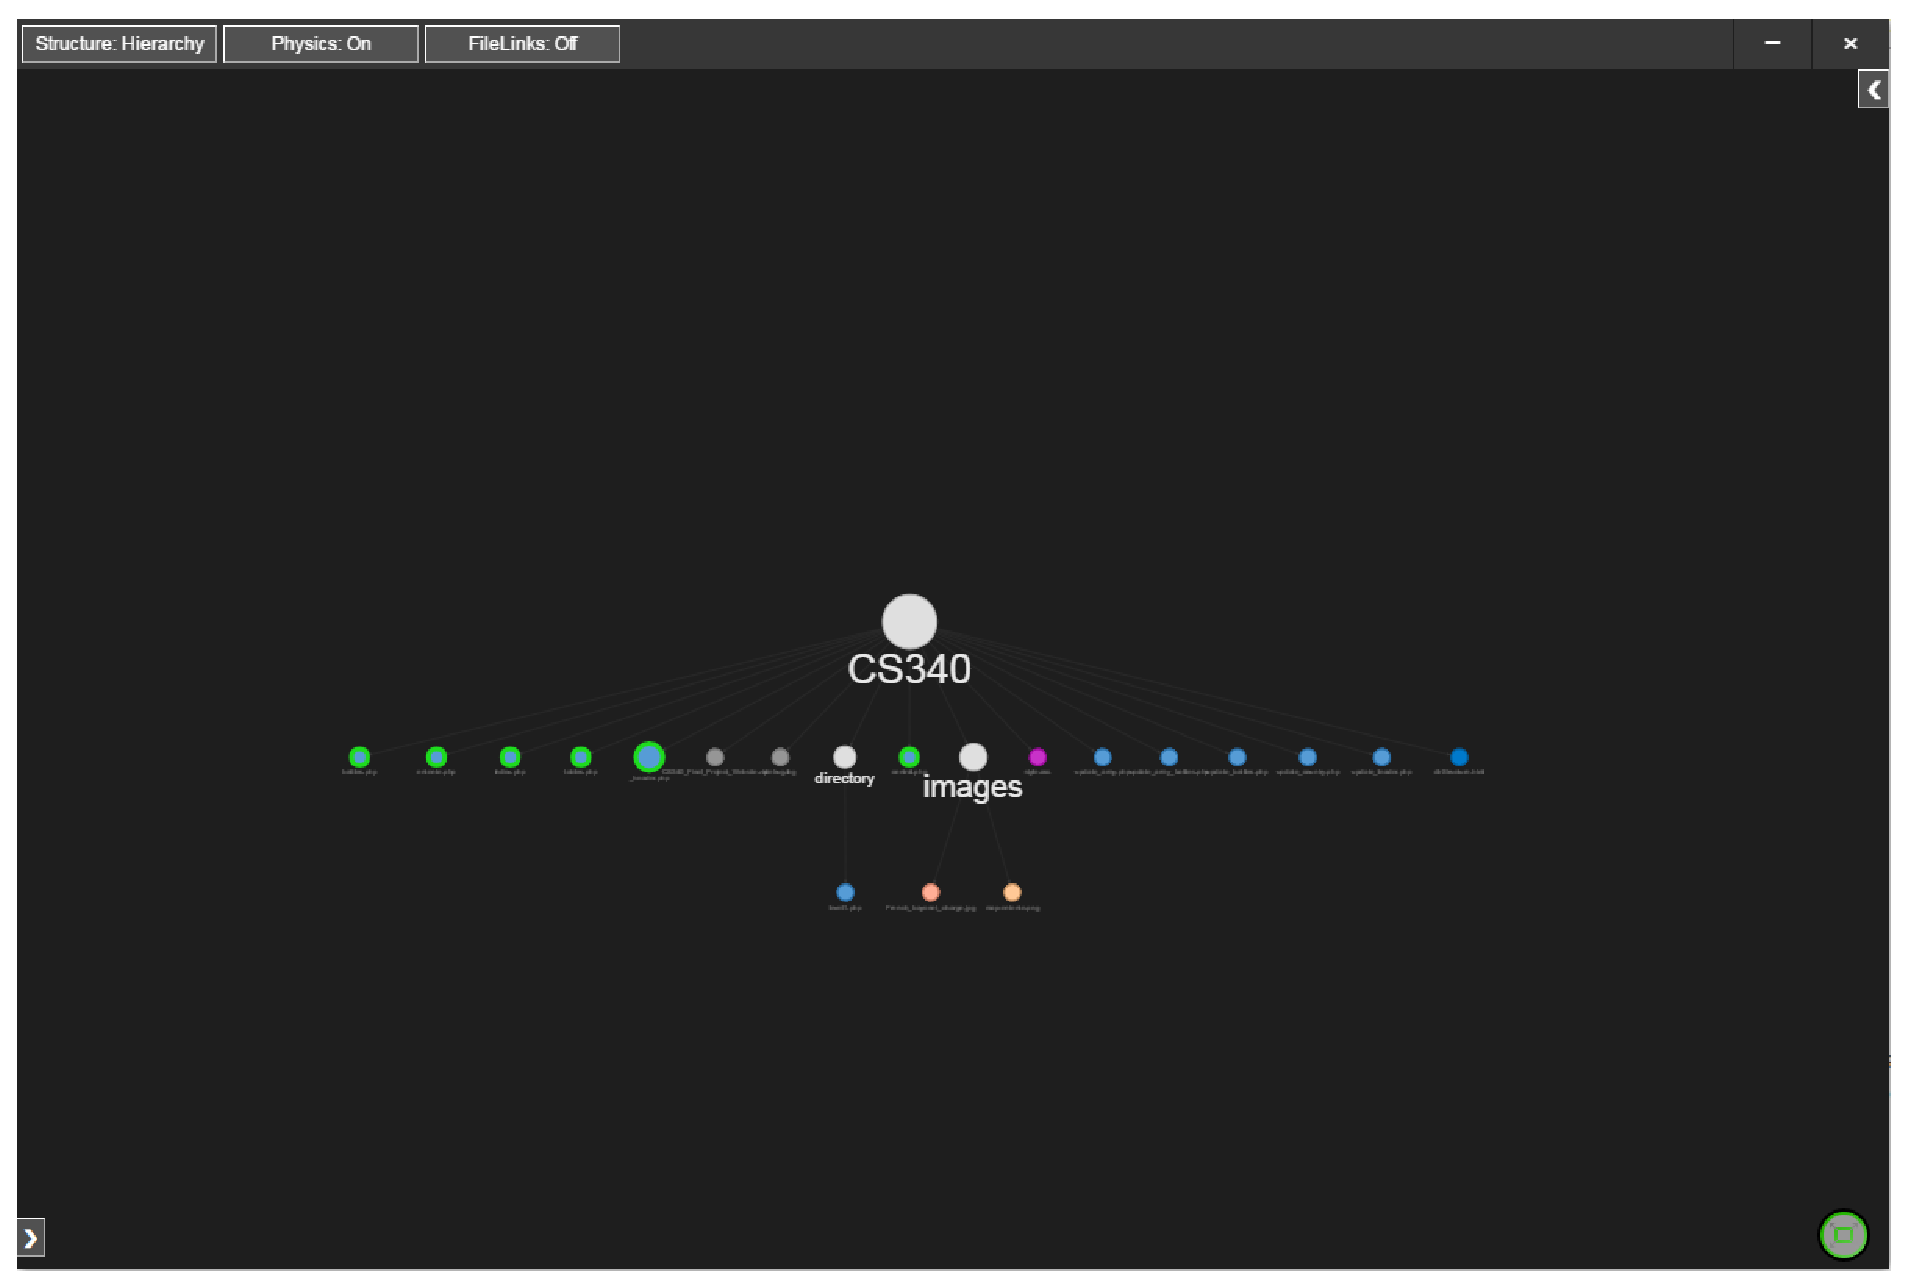
\includegraphics[width=400px]{PostalUI}
		\caption{Visualization Interface}  
	\end{figure}
	
	\begin{figure}[H]
		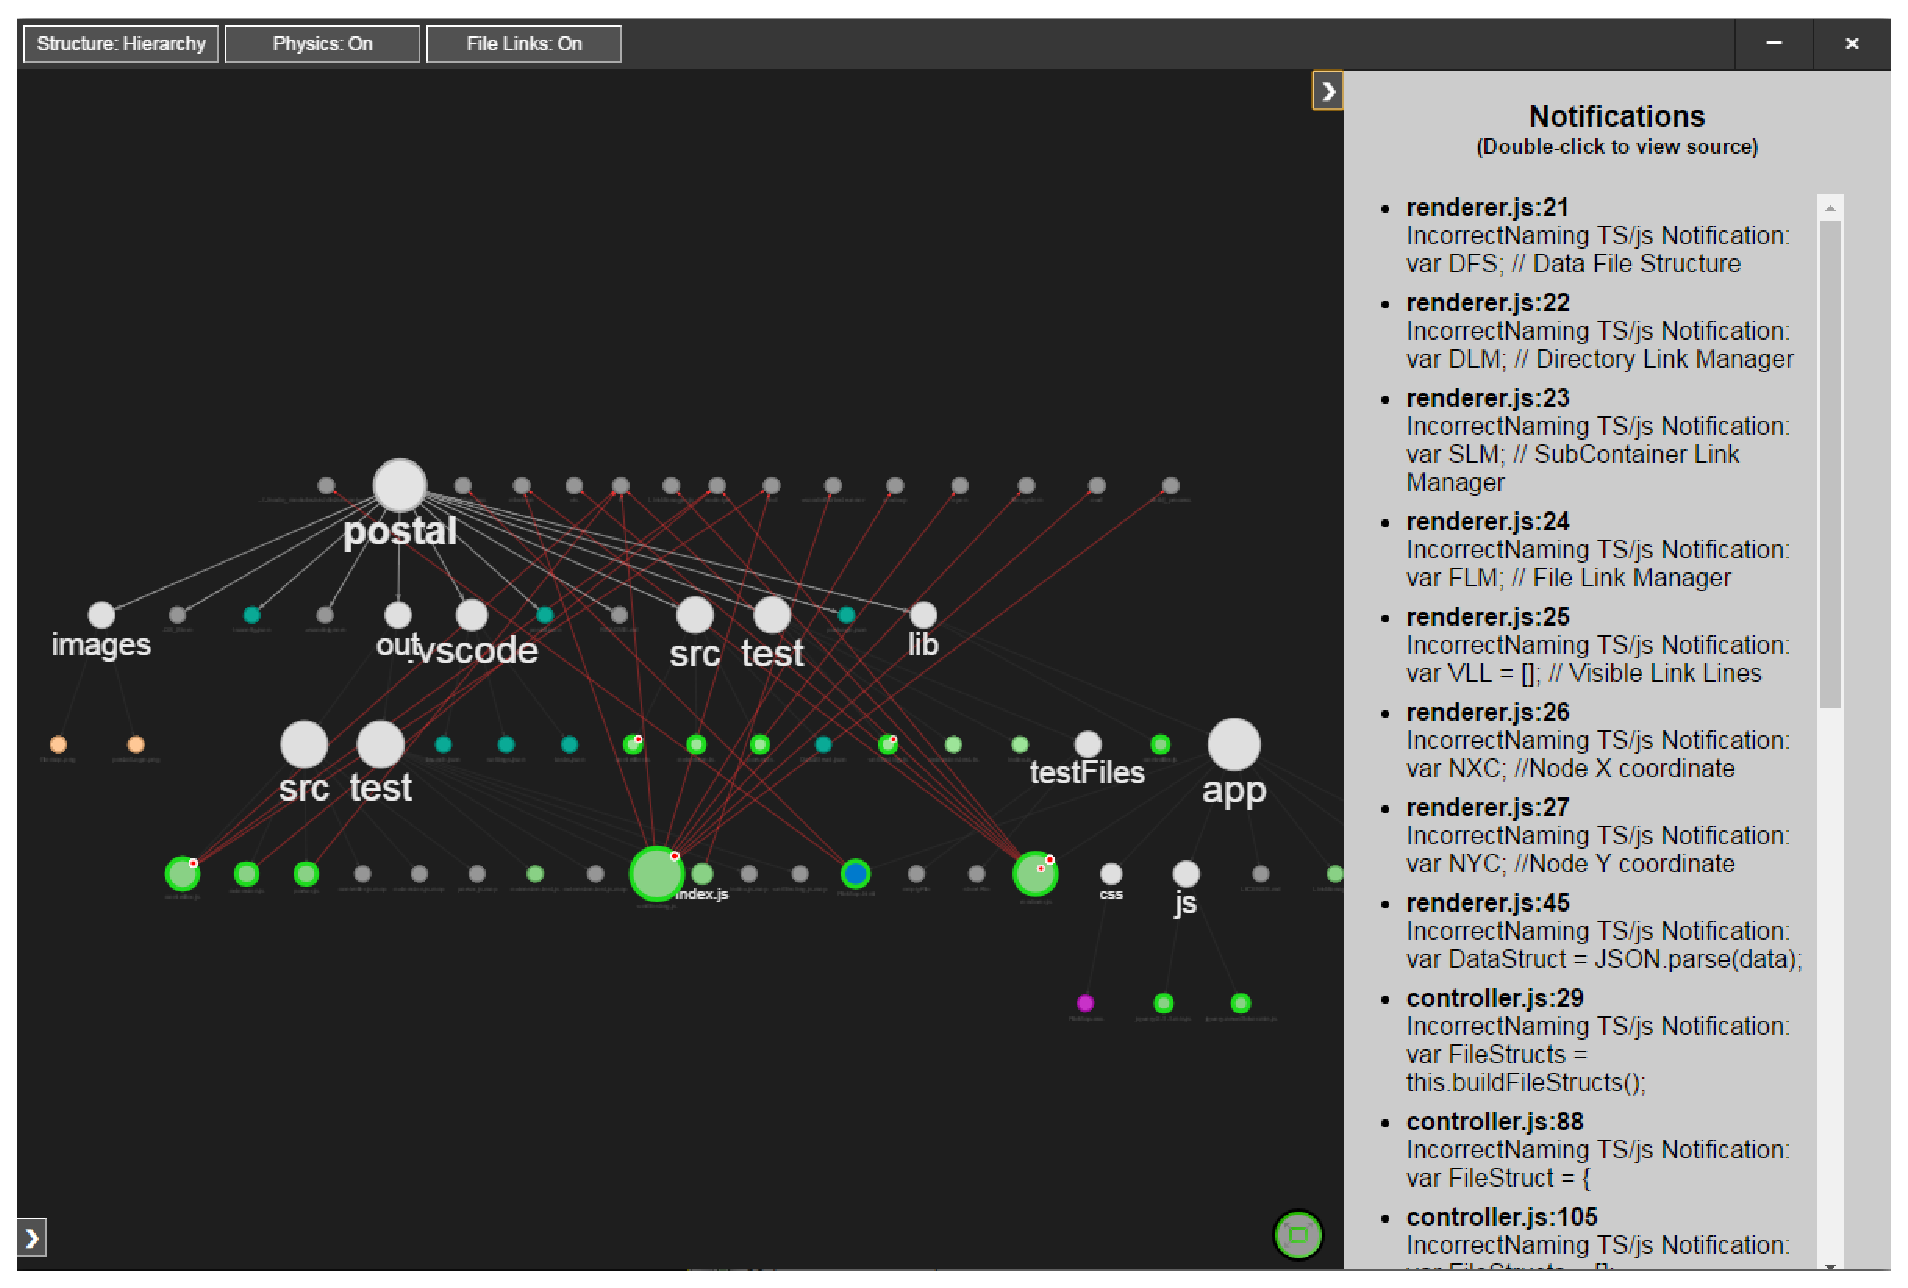
\includegraphics[width=400px]{PostalNotification}
		\caption{Notification Interface}  
	\end{figure}
	
	\begin{figure}[H]
		\includegraphics[width=400px]{UpdatedDataStruct}
		\caption{Updated Data Structure}
	\end{figure}
	
\pagebreak
\bibliographystyle{IEEEtran}
\bibliography{progress-report-team38}


\end{document}

